\documentclass[11pt,a4paper,spanish]{book} %%%Esto indica el tipo de documento.Va a ser un libro (book), el tama�o es a4, la lengua castellano (spanish)%%%
\usepackage[spanish]{babel} %%%Incluimos el paquete Babel que sirve para separar correctamente las palabras de multitud de idiomas%%%
\usepackage[latin1]{inputenc}%%%Este paquete permite poner acentos directamente%%%
\usepackage[T1]{fontenc}
\usepackage{amsmath}%%%Macros AMS%%%
\usepackage{amsthm}%%%Macros AMS para teoremas%%%
\usepackage{amsfonts}%%%Permite usar fuentes AMS%%%
\usepackage{amssymb}%%%Para usar simbolos AMS%%%
\usepackage{shadow}
\usepackage{indentfirst}%%%Espaciado deprimera l�nea de cada p�rrafo%%%
\usepackage{fancyhdr}
\linespread{1.5}
\usepackage{graphicx}
\usepackage{appendix} %%%Permite un manejo sencille de los ap�ndices. Permite tambi�n introducir subapendices.
\usepackage[colorlinks=true]{hyperref}%De esta forma el PDF sale muy chulo
\usepackage{graphics}
\usepackage{anysize} % Soporte para el comando \marginsize
\usepackage{theorem}
\usepackage{float}
\marginsize{3cm}{2cm}{2.5cm}{2.5cm}%Permite manejar los m�rgenes de forma sencilla
\usepackage[Lenny]{fncychap}
\usepackage{url}
\usepackage{eurofont}%Permite usar el s�mbolo de euro
 \pagestyle{fancy}
%\addtolength{\footskip}{+3cm}
\usepackage{fancyhdr}                                   %Para un encabezado especial m�s visual
\usepackage{extramarks}

\author{Autor 2 \and Autor 1}
\title{\textbf{\Huge{MEDIDA}}}
%-----------------------------------------------------------------------------------------------
%-----------------------------------------------------------------------------------------------
\begin{document}%%%Aqu� empieza el documento%%%

%%Portada%%
%------- T�TULO     ----------
%=============================
\begin{titlepage}
% \centerline{\bf {\large\bf D}EPARTAMENTO DE  {\large\bf T}EOR�A DE LA
% {\large\bf S}E�AL Y LAS {\large\bf C}OMUNICACIONES}
\begin{center}
{\large\textbf{UNIVERSIDAD}}
 {\large\textbf{CARLOS III DE MADRID}}\\
 \vspace{0.8cm}
{\large\textbf {ESCUELA POLIT�CNICA SUPERIOR}}\\
 \vspace{0.8cm}
{\large\textbf{INGENIER�A T�CNICA  DE TELECOMUNICACI�N}}\\
{\large\textbf {SISTEMAS DE TELECOMUNICACI�N}}
\end{center}


\begin{figure}[here]
\centering
%
\includegraphics[scale=0.3]{figuras/escudo.eps}

\includegraphics[scale=0.3]{fig/escudo.pdf}

\end{figure}


\begin{center}
{\large\textbf {PROYECTO FINAL DE CARRERA}}\\ \vspace{1.5cm}

{\Large \bf QUIERO HACER MI PFC EN \LaTeX,}\\ \vspace{0.2cm}
{\Large \bf PERO �POR D�NDE EMPIEZO?}\\ \vspace{3.5cm}
\end{center}


\begin{table}[h]
    \begin{flushright}
        \begin{tabular}{l @{\quad} l}
            \textbf{AUTOR:} & \textbf{�SCAR BARQUERO P�REZ}\\
            \textbf{TUTOR:} & \textbf{ALBERT EINSTEIN}\\
            \textbf{COTUTORA:} & \textbf{MADAME CURIE}
        \end{tabular}
        \end{flushright}
\end{table}
\begin{flushright}
{\large \textbf{19 de enero de 2005}}
\end{flushright}

\end{titlepage}
%Portada Gr�fica

\DeclareGraphicsExtensions{.jpg,.pdf,.mps,.png,.gif,.fig,.bmp}
%Declaraci�n de extensiones de figuras para el paquete graphicx

\renewcommand\tablename{Tabla}%De esta forma sale nombre de Tabla en vez de Cuadro
\renewcommand\listfigurename{Lista de Figuras}
\renewcommand\listtablename{Lista de Tablas}

\thispagestyle{empty} \cleardoublepage
%Se deja sin numeraci�n las p�ginas siguiente

%==============================================================
% Acta
%===============================================================
\thispagestyle{plain}
\begin{large}

  \noindent  \begin{tabular}{p{2cm}p{11cm}}
        \textsc{T�tulo:} & \emph{QUIERO HACER MI PFC EN \LaTeX, PERO �POR D�NDE EMPIEZO?}. \\
        & \\
        \textsc{Autor:} & \emph{�SCAR BARQUERO P�REZ} \\
        & \\
        \textsc{Tutor:} & \emph{ALBERT EINSTEIN}\\
        & \\
        \textsc{Cotutora:} & \emph{MADAME CURIE}
    \end{tabular}

\end{large}

\vspace{1cm}

La defensa del presente Proyecto Fin de Carrera se realiz� el d�a
19 de Enero de 2005; siendo calificada por el siguiente tribunal:

\vspace{0.8cm}

\noindent \begin{tabular}{p{3cm}p{10cm}}

    & \\
    \textsc{Presidente:} & \emph{Profesor Bacterio} \\
    & \\
    & \\
    \textsc{Secretario} & \emph{Mortadelo} \\
    & \\
    & \\
    \textsc{Vocal} & \emph{Filem�n} \\
\end{tabular}

\vspace{0.8cm}

Habiendo obtenido la siguiente calificaci�n:

\vspace{0.8cm}

\noindent \begin{tabular}{p{3cm}p{10cm}}

    & \\
    \textsc{Calificaci�n:} & \emph{} \\
    & \\
    \end{tabular}

\vspace{1.2cm}

\begin{bfseries}
    \begin{center}
        Presidente \hspace{3cm} Secretario \hspace{3cm} Vocal
    \end{center}
\end{bfseries}

\newpage
\thispagestyle{empty}\cleardoublepage

%==============================================================
%Agradecimientos
%==============================================================
\thispagestyle{plain}
\begin{center}
   \Large{\textbf{Agradecimientos}}
\end{center}

Agradecimientos
\newpage
\thispagestyle{empty}\cleardoublepage

%==============================================================
%Cita
%==============================================================
\thispagestyle{plain}
\newpage
\bigskip
\bigskip
\begin{flushright}
\emph{Aunque a todos les est� permitido pensar, muchos se lo
ahorran.}\\
Curts Goetx

\medskip

\emph{Te guardar�s mucho de procurarle el menor da�o a una persona
tan simp�tica y agradable como el se�or Holmes.}\\
Madre de Arthur Conan Doyle
\end{flushright}

\newpage
\thispagestyle{empty}\cleardoublepage
%==============================================================
%Resumen
%==============================================================

\chapter*{Resumen}

Aqu� ir� el resumen de tu PFC. El resumen suele constar de entre 150 y 250 palabras, con las que se da una breve introducci�n al tema que aborda el PFC, una descripci�n de lo que se propone y de los experimentos realizados, as� como una exposici�n resumida de los resultados principales y de las conclusiones.
\newpage\thispagestyle{empty}
\cleardoublepage

%===============================================================
%�ndices
%===============================================================
\pagestyle{plain}
\tableofcontents
\listoffigures
\listoftables

%===============================================================
%Para el encabezado que se va a utilizar en todo el proyecto
%===============================================================
\pagestyle{fancy}

\renewcommand{\sectionmark}[1]{\markright{\thesection\ #1}}
\fancyhf{} \fancyhead[LE,RO]{\bfseries\thepage}
\fancyhead[LO]{\bfseries\rightmark}
\fancyhead[RE]{\bfseries\leftmark}
%=============================================================

%=============================================================
%Cap�tulos
%=============================================================

\chapter{MINI TUTORIAL I}

Este documento es una plantilla para la realizaci�n del proyecto de fin de carrera (PFC), es decir, se trata de un esqueleto que facilita la labor de escribir el PFC en \LaTeX.La plantilla ha sido utilizada para escribir este mini tutorial sobre \LaTeX, de forma que tambi�n sirva de demostraci�n de c�mo utilizar los elementos m�s comunes de un PFC. El objetivo principal no es ense�ar a manejar completamente \LaTeX, si no que s�lo busca ofrecer una ayuda inicial, presentando los programas necesarios y una indicaci�n de c�mo emplearlos.


\section{Introducci�n B�sica a \LaTeX\ para Windows}

El sistema \LaTeX\  que se distribuye generalmente para Windows es el denominado MiKTeX~\cite{MiKTeX:miktex}. Es f�cilmente configurable y, adem�s, tambi�n es gratis.

\subsection{�Qu� programas necesito?}

Antes de entrar de lleno en la explicaci�n de como utilizar \LaTeX\ nos vamos a parar  en detallar cu�les son las aplicaciones necesarias y como conseguirlas:
\begin{itemize}
	\item MiKTeX: este es el sistema \LaTeX\ para Windows, se puede descargar desde: \url{www.miktex.org}. Hay que tener en cuenta que lo que te descargas desde aqu� es un instalador, que se encarga de descargar los paquetes necesarios. La instalaci�n detallada se encuentra en la siguiente secci�n.
	\item WinEdt: editor de texto para \LaTeX. Se puede descargar desde: \url{www.winedt.com}.
	\item TeXnicCenter: otro editor de texto alternativo a WinEdt. El sitio web para la descarga es: \url{www.toolscenter.org}.
	\item AFPL Ghostscript 8.51: programa interprete del lenguaje de post script (archivos .ps), que se puede descargar en: \url{www.cs.wisc.edu/~ghost/doc/AFPL/get851.htm}.
	\item GSview: visor para los archivos escritos en lenguaje post script (.ps), se puede de: \url{www.cs.wisc.edu/~ghost/gsview/}. 
	\item Acrobat Reader: aplicaci�n que permite la visi�n de archivos en formato .pdf, se puede obtener de: \url{www.adobe.es}.
\end{itemize}

Estos son los programas necesarios para poder trabajar con \LaTeX\ en Windows. Para los que est�n interesados en trabajar en sistemas Linux cabe decir que \LaTeX\ se distribuye como paquete de casi todas las distribuciones de Linux, y adem�s �stas suelen tener editores bastante buenos. Yo suelo usar Kile, que es una aplicaci�n para los escritorios KDE, parecida a los dos editores de Windows que se mencionan aqu�.

\subsection{�C�mo instalo MiKTeX?}

El primer paso es obtener una distribuci�n actualizada, cosa que se puede hacer f�cilmente en \url{http://www.miktex.org/}. 

Si optas por descarga la versi�n completa, el primer paso es bajarse un programa que se encarga de la instalaci�n cuyo nombra es \emph{setup-X}, donde \emph{X} indicar� la versi�n de la distribuci�n.

Una vez ejecutado el instalable se presenta una pantalla como la de la Figura~\ref{fig:MiktexInst}.

\begin{figure}
	\centering
		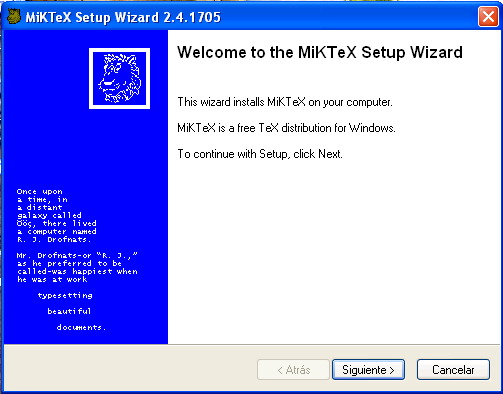
\includegraphics[width=0.60\textwidth]{fig/MiktexInst}
	\caption{\emph{Programa de instalaci�n de MiKTeX.}}
	\label{fig:MiktexInst}
\end{figure}

Este programa es un asistente de instalaci�n que permite elegir los paquetes que interesa tener y los descarga del sitio web.

Una vez pulsado el bot�n de siguiente se nos ofrece dos posibildades:
\begin{enumerate}
	\item ``Download only'': con esta opci�n, simplemente se descargan los paquetes desde Internet.
	\item ``Install'': se instalar los paquetes desde una ubicaci�n local en la que ya se tengan descargados los paquetes.
\end{enumerate}

Si estamos instalando por primera vez MiKTeX se elegir� la primera opci�n para descargar los paquetes (ver Figura~\ref{fig:MiktexInst2}).
\begin{figure}
	\centering
		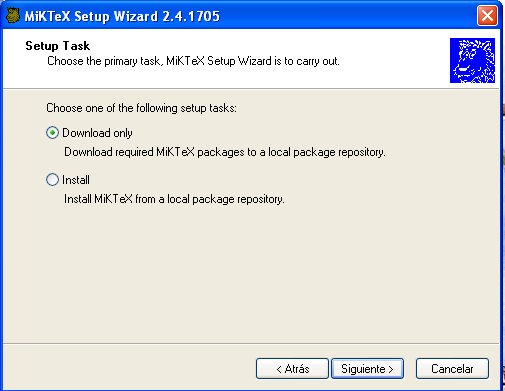
\includegraphics[width=0.60\textwidth]{fig/MiktexInst2}
	\caption{\emph{Seleccionar la opci�n de Download only.}}
	\label{fig:MiktexInst2}
\end{figure}
Una vez seleccionada la opci�n correspondiente se nos presenta una pantalla con tres opciones de instalaci�n: peque�a, grande y total, como se presenta en la Figura~\ref{fig:MiktexInst3}. La descarga total es de unos 250 MB, por lo que es recomendable tener una conexi�n de banda ancha, o bien hacerlo desde la universidad.
\begin{figure}
	\centering
		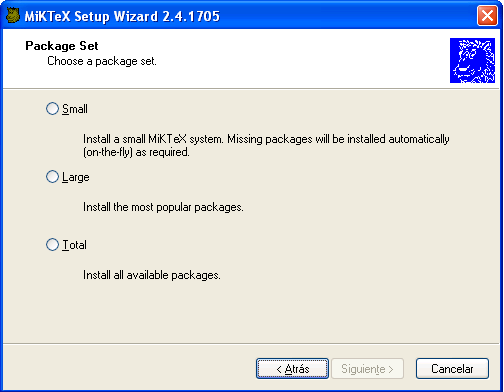
\includegraphics[width=.60\textwidth]{fig/MiktexInst3}
	\caption{\emph{La selecci�n Total implica la descarga de 250 MB.}}
	\label{fig:MiktexInst3}
\end{figure}
Independientemente de la elecci�n, es posible descargar posteriormente los paquetes necesarios.

Una vez elegido tipo de instalaci�n, se informa de los FTP's disponibles para la descarga. La elecci�n m�s adecuada es la del repositor de la rediris (Figura~\ref{fig:MiktexInst4}).

\begin{figure}[H]
	\centering
		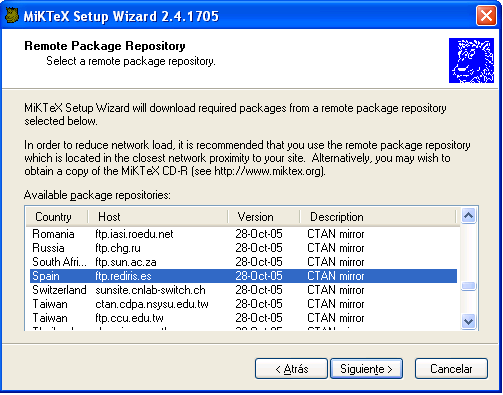
\includegraphics[width=0.60\textwidth]{fig/MiktexInst4}
	\caption{\emph{Selecci�n del repositorio de paquetes desde el que se efectuar� la descarga.}}
	\label{fig:MiktexInst4}
\end{figure}


En la pantalla, mostrada en la Figura~\ref{fig:MiktexInst5} se nos sugiere un directorio local, en nuestra m�quina, en el que se guardar�n los archivos necesarios. Este directorio simplemente sirve como repositorio local, y no corresponde al de la instalaci�n del programa MiKTeX propiamente dicha, simplemente guardar� los paquetes necesarios.

\begin{figure}
	\centering
		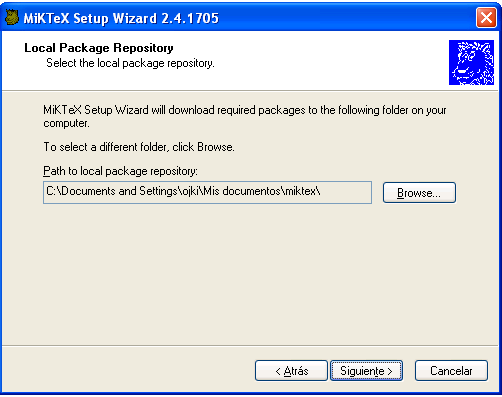
\includegraphics[width=0.60\textwidth]{fig/MiktexInst5}
	\caption{\emph{Selecci�n del directorio local donde se guardan los paquetes para la instalaci�n.}}
	\label{fig:MiktexInst5}
\end{figure}


Seguidamente se realiza la descarga. Si por alg�n motivo se suspende la descarga, se puede retomar de forma que no sea necesario realizar la descarga en una sola sesi�n (Figura~\ref{fig:MiktexInst6}).

\begin{figure}
	\centering
		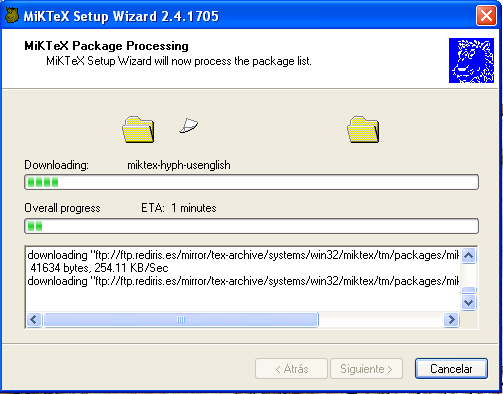
\includegraphics[width=0.60\textwidth]{fig/MiktexInst6}
	\caption{\emph{Descarga de paquetes.}}
	\label{fig:MiktexInst6}
\end{figure}


Finalmente, se notifican las elecciones que se han realizado y se procede a la instalaci�n de MiKTeX, que resulta bastante sencilla y clara. 

Siempre se pude actualizar la distribuci�n desde el men� Inicio->Programas->MiKTeX (ver Figura~\ref{fig:MiktexInst7}).
\begin{figure}
	\centering
		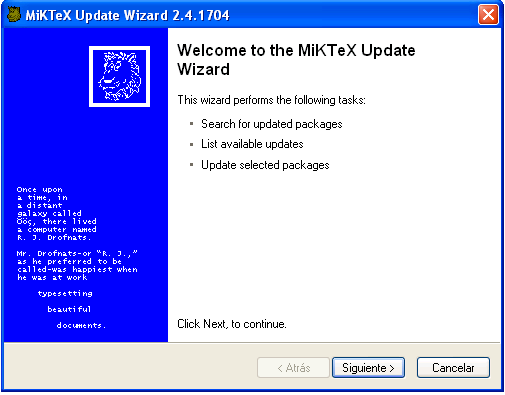
\includegraphics[width=0.60\textwidth]{fig/MiktexInst7}
	\caption{\emph{Actualizaci�n de paquetes MiKTeX.}}
	\label{fig:MiktexInst7}
\end{figure}

\subsection{Vale, pero �c�mo escribo un documento en \LaTeX?}

\subsubsection{Elegir el editor}
Los archivos que leen todos los sistemas \LaTeX\ son archivo simples de texto ASCII, con extensi�n .tex, por lo que es posible utilizar cualquier editor capaz de producir textos ASCII. Pero esto puede resultar demasiado lioso, por que implica un conocimiento de bastante amplio del funcionamiento de \LaTeX. 

Existen unos cuantos editores \LaTeX\ que se encargan de facilitar la tarea de edici�n 
A continuaci�n se detallan unos cuantos.

\begin{itemize}
	\item WinEdt~(\url{www.winedt.com}): Es un buen editor de \LaTeX, se integra muy facilmente con la distribuci�n de MiKTeX que se tenga instalada. Es bastante intuitivo y sencillo de usar. Inconvenientes: no es gratuito, se permite un uso de tiempo limitado, a partir de ese tiempo se muestra un mensaje indicando que no hemos pagado y que lo hagamos, ya que llega a resultar molesta de verdad. Existen dos posible soluciones: una es probrar suerte con los programas de libre distribuci�n y la otra es pagar la licencia. Otro problema que he encontrado es que no tiene ninguna forma de insertar figuras y tablas de forma autom�tica, aunque la soluci�n a este problema es sencilla, dado que se pueden descargar los gestores de tablas e im�genes desde la p�gina WinEdt. Para el empleo de diccionarios, y otras aplicaciones, se puede consultar tambi�n la p�gina~\url{www.winedt.org}
	
	\item TeXnicCenter~(\url{www.ToolsCenter.org}): La principal ventaja es que es gratuito, adem�s que proporciona funcionalidades similares a WinEdt, adem�s vienen integrados los gestores de tablas y figuras. El diccionario en castellano se puede conseguir mirando Tools->Options, y aqu� en la pesta�a Spelling, pulsar en el link que indica Downloads dictionar (ver Figura~\ref{fig:Texnic}).
	
	
\begin{figure}
	\centering
		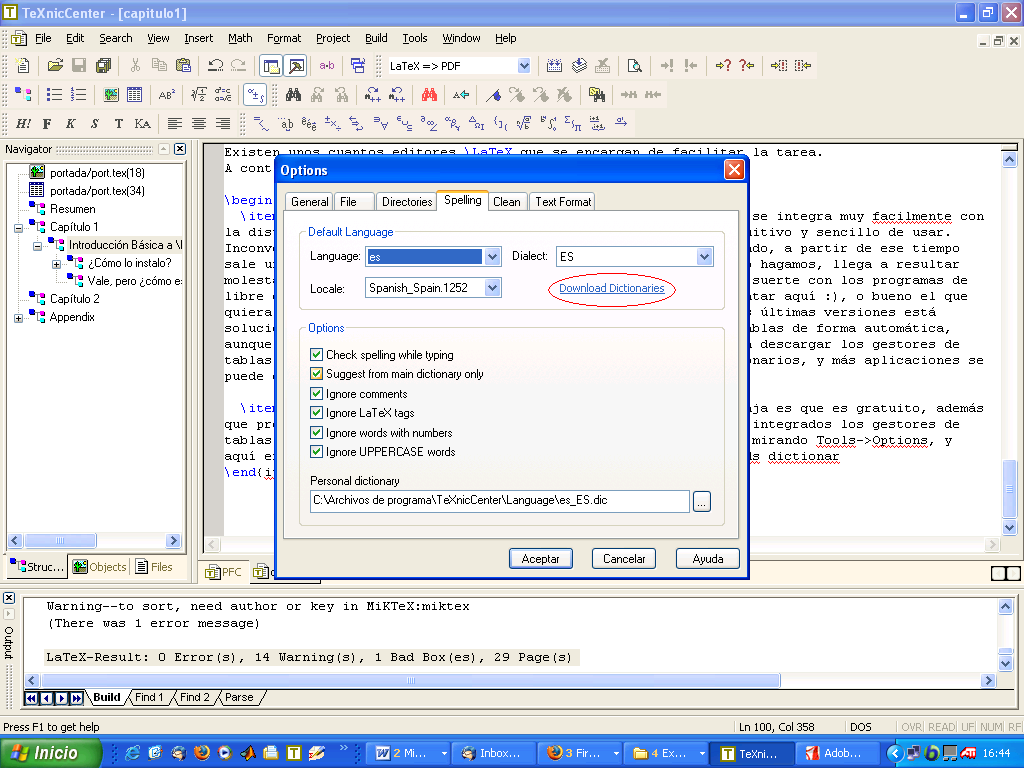
\includegraphics[width=0.75\textwidth]{fig/Texnic}
	\caption{\emph{Diccionario para TeXnicCenter.}}
	\label{fig:Texnic}
\end{figure}

Este es el editor de \LaTeX\ que yo empleo cuando trabajo en Windows.

\end{itemize}

\subsubsection{Utilizar una plantilla}

Una vez que tenemos nuestro editor y sabemos algo de \LaTeX, podemos comenzar a escribir nuestro trabajos. En general se parte de unas plantillas, por ejemplo, la que estoy empleando yo para escribir este documento. Una plantilla muy sencilla es la que se muestra a continuaci�n:
\begin{verbatim}
\documentclass[12pt,a4paper,spanish]{book} %%%Esto indica el tipo de documento.
%Va a ser un libro (book), el tama�o es a4, la lengua castellano (spanish)%%%
\usepackage{babel} %%%Incluimos el paquete Babel
	%que sirve para separar correctamente
	%las palabras de multitud de idiomas%%%
\usepackage[latin1]{inputenc}%%%Este paquete permite poner acentos directamente%%%
\usepackage{amsmath}%%%Macros AMS%%%
\usepackage{amsthm}%%%Macros AMS para teoremas%%%
\usepackage{amsfonts}%%%Permite usar fuentes AMS%%%
\usepackage[dvips]{epsfig} %%%Inclusi�n de figuras postscript
	% con visualizaci�n posterior%%%
\usepackage{indentfirst}%%%Espaciado de
	%primera l�nea de cada p�rrafo%%%
\author{Hola}
\title{Esto es un ejemplo de \LaTeX en acci�n}
\date{La fecha de hoy}
\begin{document}%%%Aqu� empieza el documento%%%
\maketitle
\tableofcontents
\listoffigures
\chapter{Primer cap�tulo}
\section{Primera secci�n}
%Texto de la secci�n
\begin {eqnarray} \label{eq1} %%%Comienzo
	%de la ecuaci�n%%%
f:A \times M \rightarrow M \\
(\lambda, x) \rightarrow \lambda x \nonumber
\end {eqnarray} %%%Fin de la ecuaci�n%%%
\end {document}

\end{verbatim}

\subsection{Compilaci�n de fuentes .tex}
Este es un ejemplo muy tonto, cuya salida es:
\begin{enumerate}
	\item Primera P�gina, Figura~\ref{fig:lat1}:
	
\begin{figure}[H]
	\centering\fbox{
		
\includegraphics[width=0.60\textwidth]{fig/lat1}}
	\caption{\emph{Salida primera p�gina.}}
	\label{fig:lat1}
\end{figure}

\item Tercera P�gina, Figura~\ref{fig:lat2}
\begin{figure}[H]
	\centering\fbox{
		
\includegraphics[width=0.60\textwidth]{fig/lat2}}
	\caption{\emph{Salida tercera p�gina.}}
	\label{fig:lat2}
\end{figure}

\item La p�gina con m�s inter�s es la s�ptima, cuya salida se muestra en la Figura~\ref{fig:lat3}

\begin{figure}[H]
	\centering
		\fbox{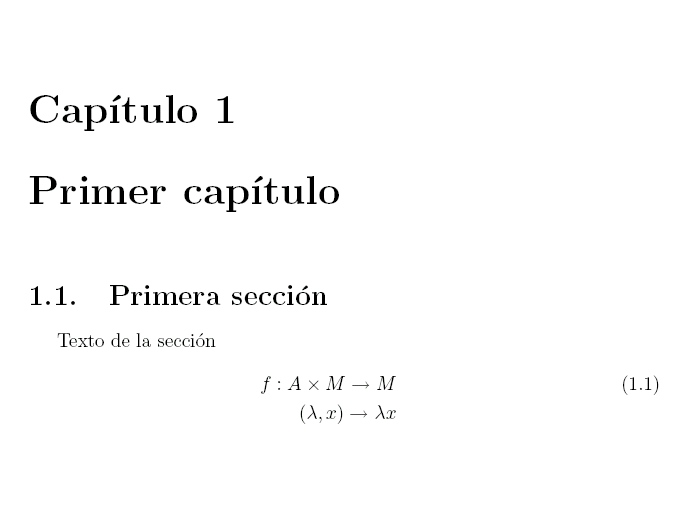
\includegraphics[width=0.60\textwidth]{fig/lat3}}
	\caption{\emph{Salida del cuerpo del texto.}}
	\label{fig:lat3}
\end{figure}

\end{enumerate}




Obviamente nos hemos saltado el paso en el que se pasa de c�gido \LaTeX, por llamarlo de alguna manera, a un fichero, que en nuestro caso era .pdf. A este proceso se le conoce como \emph{compilaci�n de fuentes}, en algunos c�rculos con el nombre de \emph{latexearlo}.

La compilaci�n se podr�a hacer por linea de comando, pero es m�s sencillo aprovechar la integraci�n de los editores con el \LaTeX\ instalado en nuestra m�quina. A continuaci�n se detalla el procedimiento para compilaci�n en los dos editores enumerados en la secci�n anterior.

Antes de pasar a la explicaci�n en cuesti�n se detallar� como obtener el visor GSViewer que para algunos casos de compilaci�n (ya se ver� cu�les) es necesario.

\subsubsection{GSview}
GSview es un interfaz gr�fico para Ghostscript. Ghostscript es un interprete para el lenguaje PostScipt usado por las impresoras laser. Para los documentos que siguen las convenciones de estructura de documentos Adobe PostScript, GSView permite seleccionar sus p�ginas para verlas o bien para imprimirlas.

Este visor necesita tener instalado el programa Aladdin GhostScript primero. 

En la web~\url{http://www.cs.wisc.edu/~ghost/gsview/Readme.htm} se detalla el procedimeinto para la instalaci�n de ambas aplicaciones, cabe mencionar que es m�s sencilla la instalaci�n si primero se intala el Aladdin GhostScript, y posteriormente el visor GSview.

\subsubsection{Compilaci�n de fuentes con WinEdt}

Existen diversas formas de compilar las fuentes, todas ellas comunes a ambos editores, por lo que se enunciar�n aqu� y no se volver�n a repetir.

\begin{enumerate}
	\item \LaTeX\ -> dvi: En esta simplemente se compilan los archivos, y se crea un archivo salida con extensi�n .dvi. Este no es un formato muy extendido para el intercambio de documentos. En WinEdt para conseguir esta compilaci�n se debe pulsar al icono en el que se se�ala la palabra \LaTeX, (ver Figura~\ref{fig:WinEdt1}).
	
\begin{figure}[H]
	\centering\fbox{
		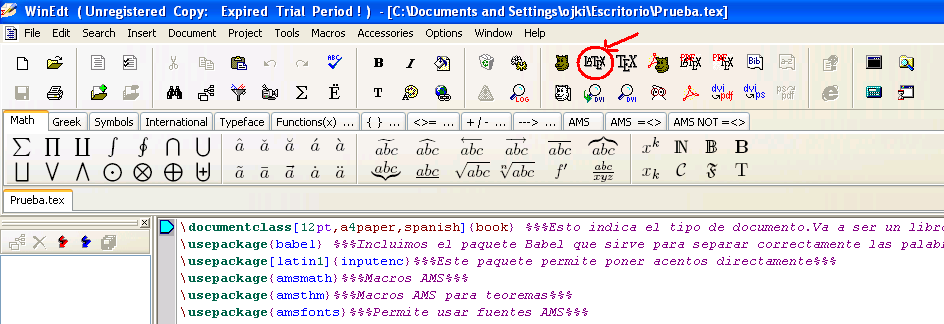
\includegraphics[width=0.85\textwidth]{fig/WinEdt1}}
	\caption{\emph{Compilaci�n a dvi con WinEdt.}}
	\label{fig:WinEdt1}
\end{figure}

A partir de aqu� se puede pasar a formato .ps, que se pueden visualizar con GSview, o bien a .pdf, que se puede visualizar con Acrobat Reader\footnote{Debemos tener instalado el Acrobat Reader en nuestra m�quina}. Para hacer esta conversi�n se emplean los iconos de WinEdt se�alados en la Figura~\ref{fig:WinEdt2}, que son bastante gr�ficos.
\begin{figure}[H]
	\centering\fbox{
		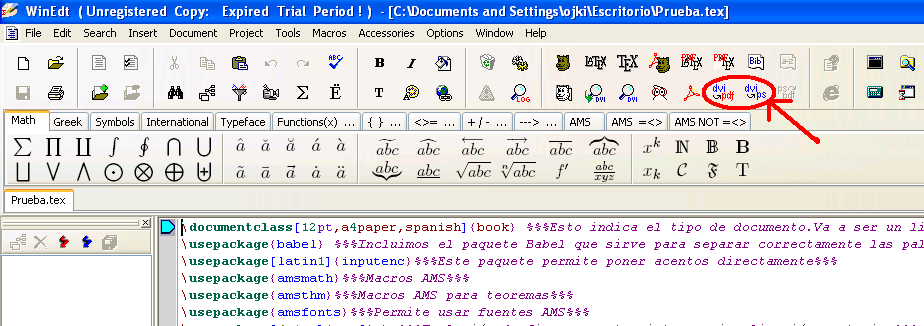
\includegraphics[width=0.85\textwidth]{fig/WinEdt2}}
	\caption{\emph{Conversi�n a formato ps o pdf.}}
	\label{fig:WinEdt2}
\end{figure}

\item \LaTeX\ -> pdf: Con esta compilaci�n directamente se obtienen las salidas en formatos pdf. El icono a emplear es el que tiene por nombre pdfLaTeX, que se muestra resaltado en la Figura~\ref{fig:WinEdt3}
\begin{figure}[H]
	\centering\fbox{
		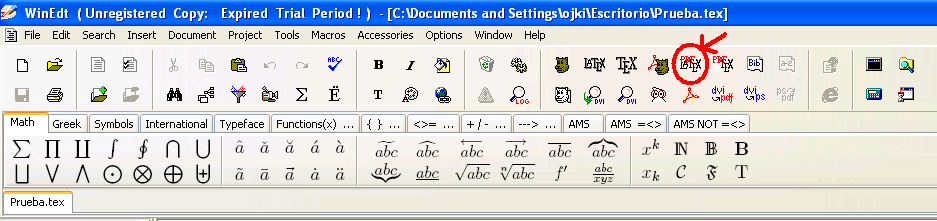
\includegraphics[width=0.85\textwidth]{fig/WinEdt3}}
	\caption{\emph{Compilaci�n Latex a pdf}}
	\label{fig:WinEdt3}
\end{figure}

En ambas compilaciones se puede emplear el icono con la mascota de \LaTeX, que est�n inmediatamente a la izquierda de los iconos mencionados, la �nica diferencia es que el empleo del icono con las mascotas lanza autom�ticamente la visi�n del documento de salida.
\end{enumerate}

En todos los casos para ver el resultado, es decir, el fichero salida que produce la compilaci�n se emplean los iconos que est�n en la fila debajo de la que contiene los iconos de compilaci�n, y que representan el logo del visor en cuesti�n. 

\subsubsection{Compilaci�n con TeXnicCenter}

La filosof�a de compilaci�n es un poco distinta, aunque fundamentalmente se realiza el mismo proceso.

En este caso s�lo existe un icono de compilaci�n, y para indicar que tipo de compilaci�n se ha de hacer en una lista desplegable de posibilidades, que se encuentra justo a la izquierda del icono de compilaci�n, (Figura~\ref{fig:Texnic1})
\begin{figure}[H]
	\centering
	\fbox{
		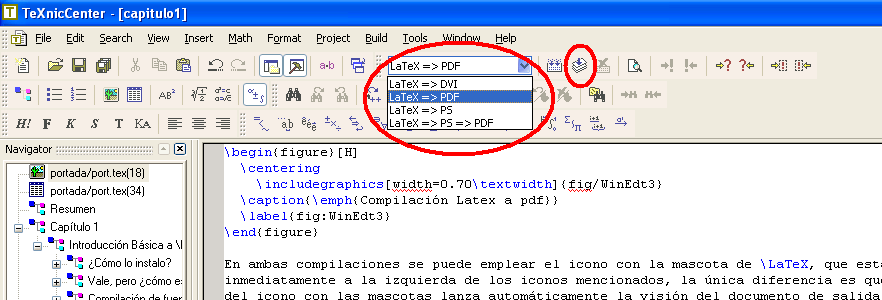
\includegraphics[width=0.85\textwidth]{fig/Texnic1}}
	\caption{\emph{Compilaci�n con TeXnicCenter.}}
	\label{fig:Texnic1}
\end{figure}

De esta forma, si nuestro objetivo es compilar a .pdf basta con indicar en el cuadro de dialogo
\begin{verbatim}
LaTeX=>PDF
\end{verbatim}

y presionar en el icono de compilar.

Para ambos editores se recomienda el uso de los proyectos, que permiten una gesti�n m�s compacta de todo un PFC por ejemplo.

\section{Un par de ideas m�s avanzadas, no mucho}

En esta secci�n se explica como incluir figuras, en distintos formatos, y tablas en \LaTeX, que en un primer acercamiento a \LaTeX\ parecen ser la parte que m�s quebraderos de cabeza da. Tambi�n se explicar� c�mo referenciar, por ejemplo, una ecuaci�n, y como incluir bibliograf�a y citas.

\subsection{Inclusi�n de figuras}

Como todo en \LaTeX, la inclusi�n de figuras se hace mediante unos comandos que indican al programa que se quiere incluir en el texto tal figura, y con una propiedades tales, y ya se encargar� el de colocarla lo mejor que pueda, seg�n lo especificado.

El problema se plantea cuando se tiene que decidir el formato de figura que se pretende insertar. Por simplificar haremos una divisi�n muy burda entre figuras eps (encapsuladas postscript) y restantes figura, tales como png, jpg, gif

La distinci�n se basa en el hecho de que la compilaci�n es distinta seg�n el grupo de figuras que se incluyan, as�:

\begin{itemize}
	\item \LaTeX->div o ps si \emph{todas} las figuras que se incluyen en el documento son eps.
	\item \LaTeX->pdf si \emph{todas} las figuras que se incluyen son de tipo png, jpg, gif. 
\end{itemize}

El procedimiento para incluir una figura en el documento es com�n a los dos grupos. En primer lugar es necesario tener incluido el paquete \emph{graphicx} en el pre�mbulo\footnote{Todo lo que hay antes de: $\backslash$begin\{document\}} con el siguiente comando:
\begin{verbatim}
	\usepackage{graphicx}
\end{verbatim}
A continuaci�n del pre�mbulo se deben declarar las extensiones que se quieren para las figuras
\begin{verbatim}
	\DeclareGraphicsExtensions{.jpg,.pdf,.png,.gif,.eps}
\end{verbatim}

En alg�n lugar cercano en el que se quiere colocar la figura se debe poner el siguiente c�digo:
\begin{verbatim}
	\begin{figure}[htbp]
    	\centering
        	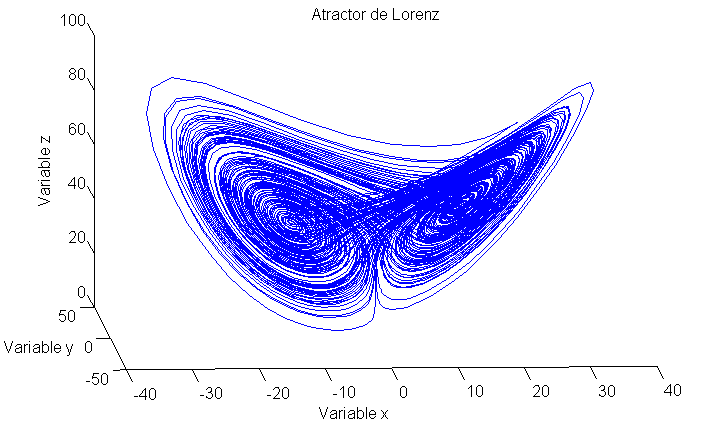
\includegraphics[width=0.60\textwidth]{fig/AtractorLorenz}
    	\caption{Mi Figura}
    	\label{fig:AtractorLorenz}
	\end{figure}
\end{verbatim}

Las opciones entre par�ntesis indican el lugar en el que se prefiere que se coloque la figura, con h se indica que aqu� (here), con t se indica que arriba (top), con b abajo (bottom) y con p en una p�gina (page) de figuras a parte. Se recomienda consultar la siguiente web \url{http://ltx.blogspot.com/2003/10/quiero-mi-figura-aqui.html}.
  
Con lo que se crea un elemento flotante figura, con el entorno \emph{figure}, que sea centrada, con \emph{centering}. 
El comando:
\begin{verbatim}
	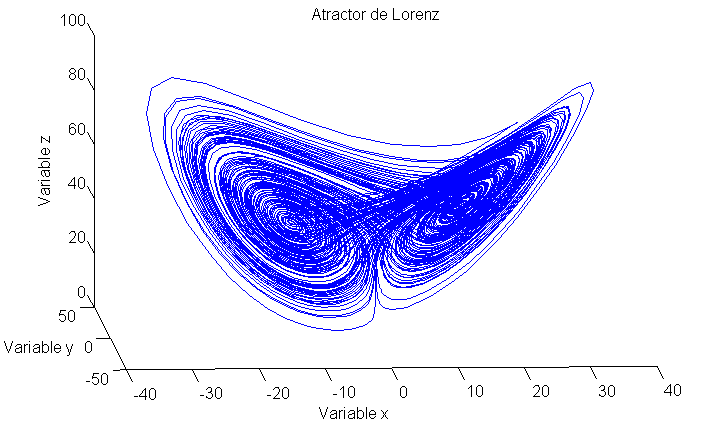
\includegraphics[width=0.60\textwidth]{fig/AtractorLorenz}
\end{verbatim}
indica que se debe colocar la figura que se tiene guardada en disco, es conveniente hacer una carpeta con todas las figuras y referenciar el path a esa figura, como se hace en el ejemplo,  que se tiene una carpeta fig en dentro de la carpeta en la que se tienen los ficheros .tex

Como se puede apreciar, no se indica la extensi�n del fichero, esta informaci�n no es necesaria, el compilador ya se encarga de buscar la extensi�n adecuada.

La informaci�n entre corchetes son opciones o modificaciones sobre el comando. En este caso se indica que se reduzca el tama�o de la figura un a un 60\% del ancho del texto que cabe en una p�gina.

Yo personalmente uso compilaci�n \LaTeX->pdf, de esta forma todas las figuras que empleo son o bien png, o bien jpg o bien gif. La elecci�n est� condicionada por el uso de estos formatos en Internet, y por lo sencillo que es tratar estos formatos con paquetes gr�ficos. Adem�s Matlab permite la obtenci�n de figuras de este estilo, mis preferidas son .png, he comprobado que la definici�n es mejor en un pdf, pero es cuesti�n de probar.

El resultado de la ejecuci�n del c�digo para la inclusi�n de la figura es el que se aprecia en la Figura~\ref{fig:AtractorLorenz}
\begin{figure}[htbp]
	\centering
		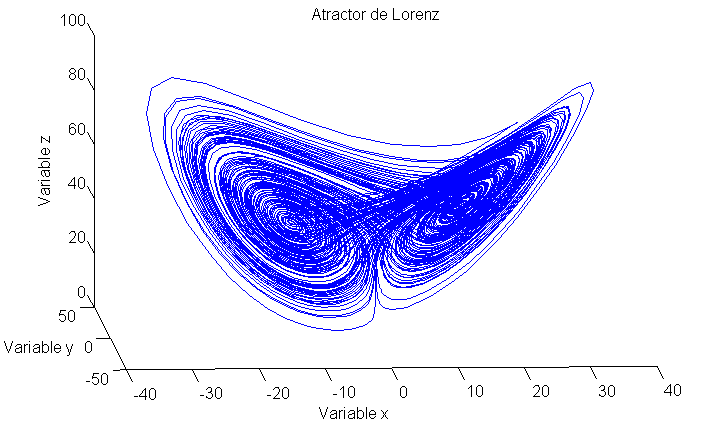
\includegraphics[width=0.60\textwidth]{fig/AtractorLorenz}
	\caption{Mi figura.}
	\label{fig:AtractorLorenz}
\end{figure}

Para cuestiones un poco m�s avanzadas sobre figuras se recomienda la siguiente p�gina: \url{http://www.udlap.mx/~ma108907/latex/figuras.html}.

\subsection{Inclusi�n de tablas}

Las tablas en \LaTeX\ tienen el objetivo principal de ser lo m�s funcionales posibles, es decir, prima el contenido frente al continente, aunque se pueden conseguir dise�os de tablas muy est�ticos, pero hay que tener en cuenta esto. La filosof�a de la inclusi�n de tablas es similar a la de la inclusi�n de figuras, dado que primero se crea un entorno flotante, en este caso de tabla, y dentro de �l se crea la tabla que deseemos. Un ejemplo sencillo ser�a:
\begin{verbatim}
	\begin{table}[h]
	\scriptsize
  	  \begin{tabular}{|l|c|l|}
    	\hline
    	\textbf{Variable}& \textbf{Unidades} & \textbf{Descripci�n}\\
    	\hline
    	\hline
    	HRV index & ms & N�mero total de intervalos RR dividido por la altura del\\
    	& & histograma de todos los intervalos RR usando celdas de 8 ms.\\
    	TINN & ms & Anchura de la l�nea de base de la interpolaci�n triangular,\\
    	& & diferencia de m�nimos cuadrados, del pico m�s alto del\\
    	& & histograma de todos los intervalos RR.\\
    	Dispersi�n del diagrama de Lorenz & ms & \\
    	& & intervalos RR frente a la de los anteriores.\\
    	\hline
    	\hline
    	\end{tabular}
    	\caption{\emph{M�todos geom�tricos: medidas temporales de la HRV.}}
    	\label{tab:MedidasTemporalesGeometricas}
	\end{table}
\end{verbatim}

Las letras entre par�ntesis al lado del comando 
\begin{verbatim}
	\begin{tabular}
\end{verbatim}

indican la alineaci�n que tendr�n los elementos de las respectivas columnas, en este caso los de la primera columna estar�n alineados a la izquierda, al igual que los de la tercera columna, mientras que los de la segunda estar�n centrados.

El resultado de esta se muestra en la Tabla~\ref{tab:MedidasTemporalesGeometricas}

\begin{table}[h]
\scriptsize
    \begin{tabular}{|l|c|l|}
    \hline
    \textbf{Variable}& \textbf{Unidades} & \textbf{Descripci�n}\\
    \hline
    \hline
    HRV index & ms & N�mero total de intervalos RR dividido por la altura del\\
    & & histograma de todos los intervalos RR usando celdas de 8 ms.\\
    TINN & ms & Anchura de la l�nea de base de la interpolaci�n triangular,\\
    & & diferencia de m�nimos cuadrados, del pico m�s alto del\\
    & & histograma de todos los intervalos RR.\\
    Dispersi�n del diagrama de Lorenz & ms & Mapa de puntos en el que se representa la duraci�n de los\\
    & & intervalos RR frente a la de los anteriores.\\
    \hline
    \end{tabular}
    \caption{\emph{M�todos geom�tricos: medidas temporales de la HRV.}}
    \label{tab:MedidasTemporalesGeometricas}
\end{table}

\subsection{Referencias}

El manejo de referencias en \LaTeX\ es una de sus principales ventajas, dado que nosotros no debemos mantener un control total de la numeraci�n, simplemente se debe hacer un peque�o ejercicio de orden a la hora de organizar las etiquetas (labels), y las referencias.

Para poder referenciar cap�tulos, secciones (en general cualquier apartado del documento), figuras, tablas, ecuaciones, etc. primero se deben etiquetar. Para ello se emplea el comando 
\begin{verbatim}
	\label{}
\end{verbatim}

Una recomendaci�n es la de emplear las etiquetas de la siguiente forma: se divide la etiqueta con 
\begin{verbatim}
	\label{part1:part2}
\end{verbatim}

En part1 se colocar� la naturaleza de lo que se quiere referenciar, si se trata de una secci�n ser� sec, si es una figura ser� fig, etc. En part2 se debe indicar un nombre representativo de lo referenciado, as� si es una figura que representa el atractor de Lorenz, la etiqueta completa ser�:
\begin{verbatim}
	\label{fig:AtractorLorenz}
\end{verbatim}

La manera de hacer referencia de esta figura basta con incluir el siguiente c�digo:
\begin{verbatim}
	\ldots como se puede observar en la Figura~\ref{fig:AtractorLorenz}.
\end{verbatim}

Lo que una vez compilado resulta ser:


\medskip
\shabox{... como se puede observar en la Figura~\ref{fig:AtractorLorenz}.}
\medskip

\subsection{Bibliograf�a}

Este es otro de los apartados m�s rese�ables de \LaTeX. Existen diversas formas de introducir la bibliograf�a en un documento. En este apartado se introduce el uso de BibTeX, herramienta que permite un sencillo manejo de una amplia bibliograf�a como puede ser la que se ha de emplear en un PFC.

El primer paso es crear un archivo .bib, que no es nada m�s ni menos que un archivo de texto con la terminaci�n .bib, esto se puede hacer con los propios editores de \LaTeX, en este aspecto WinEdt le lleva ventaja a TeXnicCenter. 

Este archivo no es m�s que un conjunto de entradas como la que se muestra a continuaci�n:
\begin{verbatim}
@article{HRV:Bezerianos95,
 author = "A. Bezerianos and G. Papaioannou and P. Polydoropoulos",
 title = "Nonlinear time series analysis of electrocardiograms",
 journal = "Chaos",
 volume = "5",
 number = "1",
 pages = "95--101"
}
\end{verbatim}

Con WinEdt es tan sencillo como insertar un item de BibTeX, lo que se puede realizar como se muestra en la Figura~\ref{fig:WinEdt4}
\begin{figure}[htbp]
	\centering
		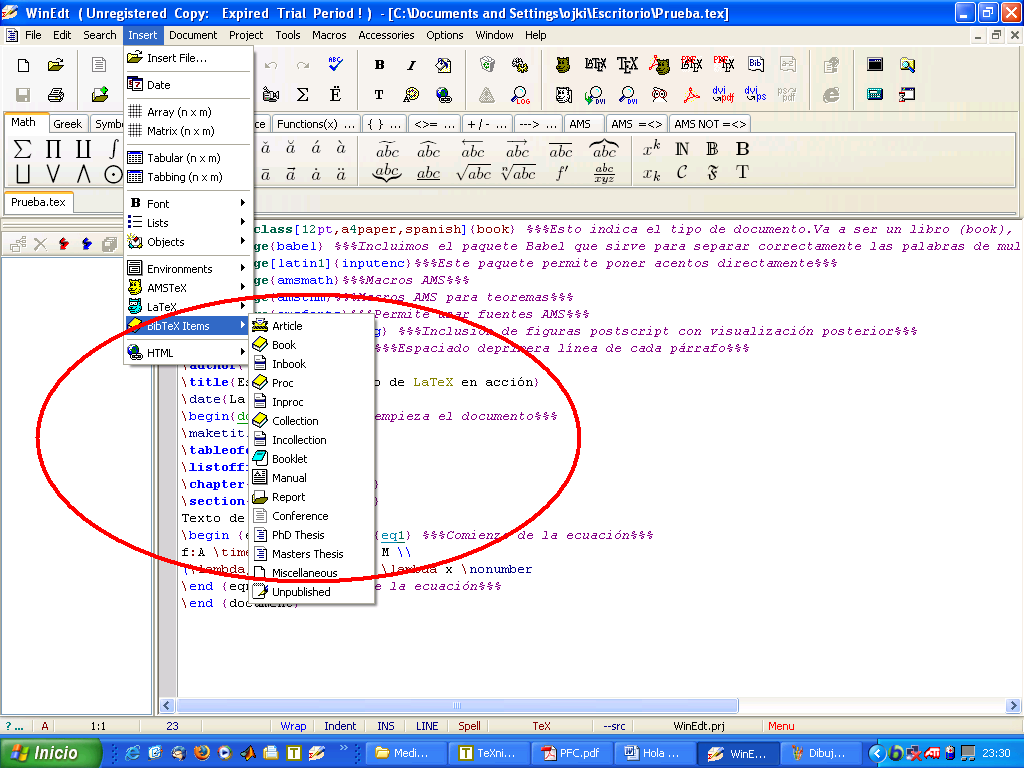
\includegraphics[width=0.85\textwidth]{fig/WinEdt4}
	\caption{\emph{Selecci�n de una nueva entrada para BibTeX}}
	\label{fig:WinEdt4}
\end{figure}

Para citar el art�culo anterior en el documento que estemos escribiendo, primero se debe introducir los siguientes comandos en el archivo .tex principal:
\begin{verbatim}
\bibliographystyle{abbrv}
\bibliography{bsample}
\end{verbatim}

El primer comando indica el estilo que se emplear� en la bibliograf�a, y el segundo el archivo en el que est� esa bibliograf�a.

En la zona exacta en la que se quiere citar, se debe colocar la siguiente sentencia:
\begin{verbatim}
\ldots para ampliar los conceptos expuestos, consultar~\cite{HRV:Bezerianos95}.
\end{verbatim}

Como se puede apreciar, se debe seguir un cierto orden para las entradas de las citas. Compilado lo anterior queda:

\medskip
\shabox{\ldots para ampliar los conceptos expuestos, consultar~\cite{HRV:Bezerianos95}.}
\medskip

Para que la compilaci�n tenga �xito, en el editor WinEdt es necesario primero utilizar el icono ``Bib'', (ver Figura~\ref{fig:WinEdt5}). Esto permite ejecutar la herramienta BibTeX, si bien probablemente ser� necesario hacerlo un par de veces para actualizar todas las citas, y posteriormente latexear el documento entero.

\begin{figure}[htbp]
	\centering
		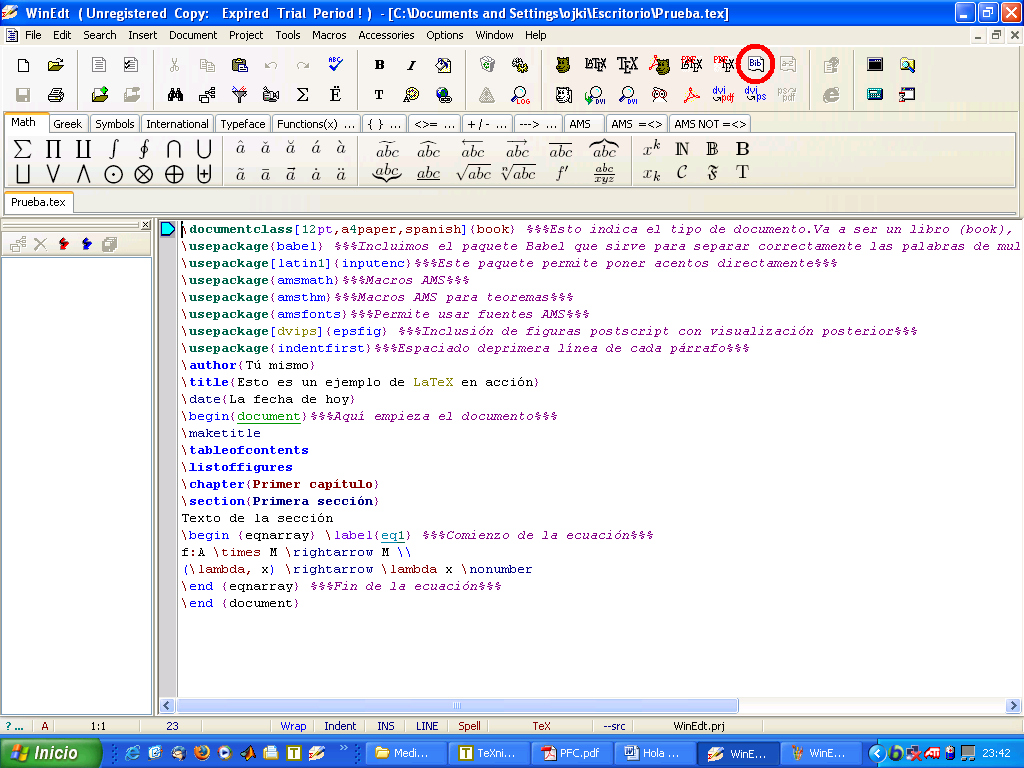
\includegraphics[width=0.85\textwidth]{fig/WinEdt5}
	\caption{\emph{Compilaci�n del BibTeX.}}
	\label{fig:WinEdt5}
\end{figure}

En el editor TeXnicCenter basta simplemente con compilar unas cuantas veces, al menos dos veces para que el programa sea capaz de actualizar todas las referencias.

\section{Conclusiones y recomendaciones}

Este peque�o tutorial no pretende ense�ar el manejo de la potente herramienta que es \LaTeX\, si no simplemente ayudar a superar el miedo inicial ante un nuevo lenguaje que permite crear textos muy bien estructurados y, sobre todo, que permite el manejo de documentos de extensi�n larga. 

Nos ha parecido interesante resumir en un mismo documento los pasos iniciales antes de poder usar \LaTeX, tales como la instalaci�n y el manejo b�sico de las herramientas necesarias, as� como peque�os ejemplos de ciertos aspectos que al principio pueden resultar muy extra�os para los que venimos del mundo Word. 

Con lo aqu� expuesto no se pueden crear documentos, pero permite un acercamiento amigable, que unido a la consulta de los libros y documentos que a continuaci�n se presentan permitir�an llegar a tener un control aceptable de \LaTeX.

Se recomeniendan como referencias para el manejo de \LaTeX:
\begin{itemize}
	\item The LaTeX Companion. Libro que se encuentra en la biblioteca.
	\item ~\url{www.cervantex.org}. Magnifico sitio Web, muy recomendable.
	\item \textit{The not so shot introduction to LaTeX}. Se encuentra en Internet de forma gratuita.
\end{itemize}

Aparte de infinidad de informaci�n que se pude encontrar con solo introducir en el buscador de Google la palabra  \LaTeX.
\chapter{MINI TUTORIAL II}


%============================================================
%   Ap�ndices
%============================================================
\renewcommand{\appendixtocname}{AP�NDICES}%Cambia el nombre de toc para ap�ndices
\renewcommand{\appendixpagename}{AP�NDICES}%Cambia el nombre para la p�gina
\renewcommand{\appendixname}{AP�NDICE}
\appendix
\appendixpage
\addappheadtotoc
\chapter{PRESUPUESTO DEL PROYECTO}
En este ap�ndice se presentan justificados los costes globales de
la realizaci�n de este Proyecto Fin de Carrera. Tales costes,
imputables a gastos de personal y de material, se pueden deducir
de las Tablas~\ref{tab:presupuesto1} y~\ref{tab:presupuesto2}.

\begin{sf}
    \begin{table}
        \begin{center}
            \caption[Fases del Proyecto]{\it\small \label{tab:presupuesto1} Fases del Proyecto}
            \vspace{2pt}
            \fbox{\begin{tabular}{|c|c|c|}


                \hline
                \emph{\textbf{Fase 1}} & \emph{Documentaci�n} & $350$ \emph{horas} \\
                \hline
                \emph{\textbf{Fase 2}} & \emph{Desarrollo del software} & $90$ \emph{horas} \\
                \hline
                \emph{\textbf{Fase 3}} & \emph{An�lisis de la base de datos} &  $500$ \emph{horas} \\
                \hline
                \emph{\textbf{Fase 4}} & \emph{Redacci�n de la memoria del proyecto} & $250$ \emph{horas} \\
                \hline

            \end{tabular}}
        \end{center}
    \end{table}
\end{sf}

En la Tabla~\ref{tab:presupuesto1} se muestran las fases del
proyecto y el tiempo aproximado para cada una de ellas. As� pues,
se desprende que  el tiempo total dedicado por el proyectando ha
sido de 1.190 horas, de las cuales aproximadamente un 30\% han
sido compartidas con el tutor del proyecto, por lo que el total
asciende a 1.547 horas. Teniendo en cuenta que la tabla de
honorarios del Colegio Oficial de Ingenieros T�cnicos de
Telecomunicaci�n establece unas tarifas de 60 \euro$/$hora, el
coste de personal se sit�a en 92.820 \euro.

\begin{sf}
    \begin{table}
        \begin{center}
            \caption[Costes de material]{\it\small \label{tab:presupuesto2} Costes de material}
            \vspace{2pt}
            \fbox{\begin{tabular}{|c|c|}


                \hline
                \emph{Ordenador de gama media} & 1.300 \euro \\
                \hline
                \emph{Local (durante 12 meses, con un coste de 120 \euro/mes}) & 1.440 \euro \\
                \hline
                \emph{Documentaci�n} & 200 \euro \\
                \hline
                \emph{Gastos varios} & 700 \euro \\
                \hline

            \end{tabular}}
        \end{center}
    \end{table}
\end{sf}

En la Tabla~\ref{tab:presupuesto2} se recogen los costes de
material desglosados en equipo inform�tico, local de trabajo,
documentaci�n y gastos varios no atribuibles (material fungible,
llamadas telef�nicas, desplazamientos...). Ascienden, pues, a un
total de 3.640 \euro.

A partir de estos datos, el presupuesto total es el mostrado en la
Tabla~\ref{tab:presupuesto3}.

\begin{sf}
    \begin{table}
        \begin{center}
            \caption[Presupuesto]{\it\small \label{tab:presupuesto3} Presupuesto}
            \vspace{2pt}
            \fbox{\begin{tabular}{|c||c|}


                \hline
                \textbf{Concepto} & \textbf{Importe} \\
                \hline
                Costes personal & 78.000 \euro \\
                \hline
                Costes material & 3.640 \euro \\
                \hline
                Base imponible & 96.460 \euro\\
                \hline
                I.V.A. ($16\%$) & 15.433,6 \euro \\
                \hline
                TOTAL & 111.893,6 \euro \\
                \hline

            \end{tabular}}
        \end{center}
    \end{table}
\end{sf}


%------------------------------------------------------------
%          Bibliografia
%------------------------------------------------------------
\bibliographystyle{abbrv}
\bibliography{bsample}
%-------------------------------------------------------------

\end{document}
